\scanpage{15}
\figure{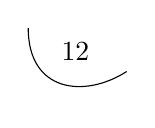
\begin{tikzpicture}[x=1cm,y=1cm]
\node at (0,0) {\mspage{12}};
\draw (-.6,.3) .. controls (-.6,-.5) and (.1,-.6) .. (.65,-.25);
\end{tikzpicture}}
\deleted{\unsure{Donc le}} $\Phi_0$ est un module libre sur $\mathbb Z$, engendré par les
\[
\varphi_i^{\beta,\alpha}\quad\deleted{\unsure{\pi_{i\alpha}}}\qquad 0\leq i\leq n,\quad0\leq\alpha,\beta\leq2n-i
\]
\deleted{\[
\left\{\quad\unsure{L^j|L^\beta}\pi_{i,\alpha}\quad\varphi_{i,\alpha}^{j,\beta}\quad\unsure{\pi_{i\alpha}}\quad\text{pour}\quad
\left\{\begin{aligned}
\unsure{i,j}\quad0\leq i\leq2n,\ 0\leq j\leq2n,\ \alpha,\beta\geq0\\
i-2\alpha=j-2\beta\geq0\\
\unsure{i<j}
\end{aligned}\right.\right.
\]}
\margin{$\mathbb Z$ \unsure{peut} être remplacé par n'importe quel anneau}
\deleted{$\varphi_{i,\alpha}^{j,\beta}$ est nul sur les composantes}
définis par
\inserted{\[
\left|\begin{aligned}
\varphi_i^{\beta\alpha}&=L_0^{\beta-\alpha}\pi_{i+2\alpha,\alpha}\quad\text{si }\alpha\leq\beta\\
\varphi_i^{\beta\alpha}&=\Lambda_0^{\alpha-\beta}\pi_{i+2\alpha,\alpha}\quad\text{si }\alpha\geq\beta\quad\deleted{\unsure{\beta-\alpha|\beta\leq\alpha}}
\end{aligned}\right.
\]}
\deleted{\[
\left\{\begin{aligned}
\varphi_{i,\alpha}^{j,\beta}&=L_0^{\beta-\alpha}\pi_{i,\alpha}=\pi_{j,\beta}L_0^{\beta-\alpha}\quad\text{si }\alpha\leq\beta\\
\varphi_{i,\alpha}^{j,\beta}&=\Lambda_0^{\alpha-\beta}\pi_{i,\alpha}=\pi_{j,\beta}\Lambda_0^{\alpha-\beta}\quad\text{si }\alpha\geq\beta
\end{aligned}\right.
\]}
i.e. on a une base formée des
\deleted{\[
\left\{L^\beta\pi_{i,\alpha}\quad\left\{\begin{aligned}
0\leq i\leq\unsure{2n|n},\quad\alpha\geq0\quad\text{donc }i-2\alpha\geq0\\
0\leq2\alpha\leq i\\
0\leq\beta
\end{aligned}\right.\right.
\]}
\margin{\[
\varphi_{i'}^{\beta',\alpha'}\varphi_i^{\beta,\alpha}\unsure{=}\left\{\begin{array}{ll}
0&\text{si }\deleted{\unsure{i-2\alpha\neq j-2\beta}}\inserted{i\neq i'\text{ ou }\beta\neq\alpha'}\\
\varphi_i^{\beta',\alpha}\deleted{\unsure{\alpha'}}&\text{sinon}
\end{array}\right.
\]
\deleted{$\unsure{\varphi_{i,\alpha}^{j,\beta}\varphi_{i',\alpha'}^{j',\beta'}=}$}}
\margin{\figure{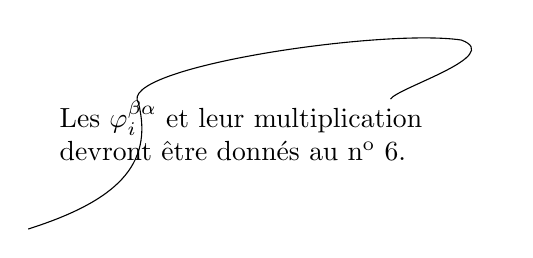
\begin{tikzpicture}
\node[align=left,text width=4.8cm,inner sep=8pt] (a) at (0,0) {Les $\varphi_i^{\beta\alpha}$ et leur multiplication \unsure{devront} être donnés au n\textsuperscript{o} 6.};
\draw (-2.8,-1.25) .. controls (-1.7,-.9) and (-1.2,-.45) .. (-1.4,.35) .. controls (-1.7,.8) and (1.7,1.3) .. (2.7,1.15) .. controls (3.25,.95) and (1.9,.55) .. (1.8,.4);
\end{tikzpicture}}}

La multiplication des bases \unsure{ne} bien sûr dépend pas du choix de $\mathbf M_0,\xi_0$ (\unsure{qui au fond} \unsure{unique est} sur l'anneau $\mathbb Z$ ....), donc l'anneau $\Phi_0$ est bien déterminé en termes de l'entier \inserted{\figure{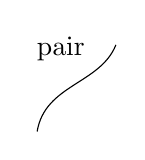
\begin{tikzpicture}[x=1cm,y=1cm]
\node at (0,.35) {pair};
\draw (-.3,-.7) .. controls (-.2,-.1) and (.5,-.1) .. (.7,.4);
\end{tikzpicture}}} $2n$.

\uline{Proposition} Revenant à la donnée de $M^*$ comme au n\textsuperscript{o} 6, et de $\mathcal E$ \deleted{\unsure{sous-algèbre}}\inserted{anneau} gradué de \deleted{$\unsure{\mathcal E}$} $\operatorname{End}(M^*)$.
\inserted{Soit $L\in\mathcal E^{(2)}$}
Conditions équivalentes

(i) L'\unsure{endom} $L$ de $M^*$ satisfait la condition de \deleted{Hard} Lefschetz et l'opérateur $\Lambda$ associé est dans $\mathcal E$.
(c. à d. on est dans les conditions du th. du n\textsuperscript{o} 6).

\unsure{(iii)|(ii)} Il existe un hom d'anneaux gradués
\[
\varphi:\Phi_0\longrightarrow\mathcal E
\]
\mspage{14}
